\chapter[LTL Language]{The Language to specify LTL Properties: a reference}
\label{language}
\index{LTL Language}

\section{Introduction}
\label{language:introduction}

Using the Default LTL Checker plugin or the LTL Checker plugin with
LTL Template files created by others is easy as you have read in the previous
chapter. Writing your own LTL Template files is another matter. This chapter
tries to give a full and complete overview of the LTL Language, so that you
can specify your own LTL properties.

Before the language itself is explained, the environment the language operates
in is given.

\section{The Environment in which the Language operates}
\label{language:environment}
\index{LTL language!Environment}

The LTL Language specifies properties of workflow logs of processes. A process
can be seen as a list of $N$ process instances. Every process instance itself
is a list of $M$ ordered audit trail entries ( Figure \ref{language:log}).
Actual $M$ can be different for any process instance. Both audit trail entries and
process instances can have data fields. About audit trail entries we know that
there are always a WorkflowModelElement and an EventType data field, other fields are permitted too.

\begin{figure}[H]
    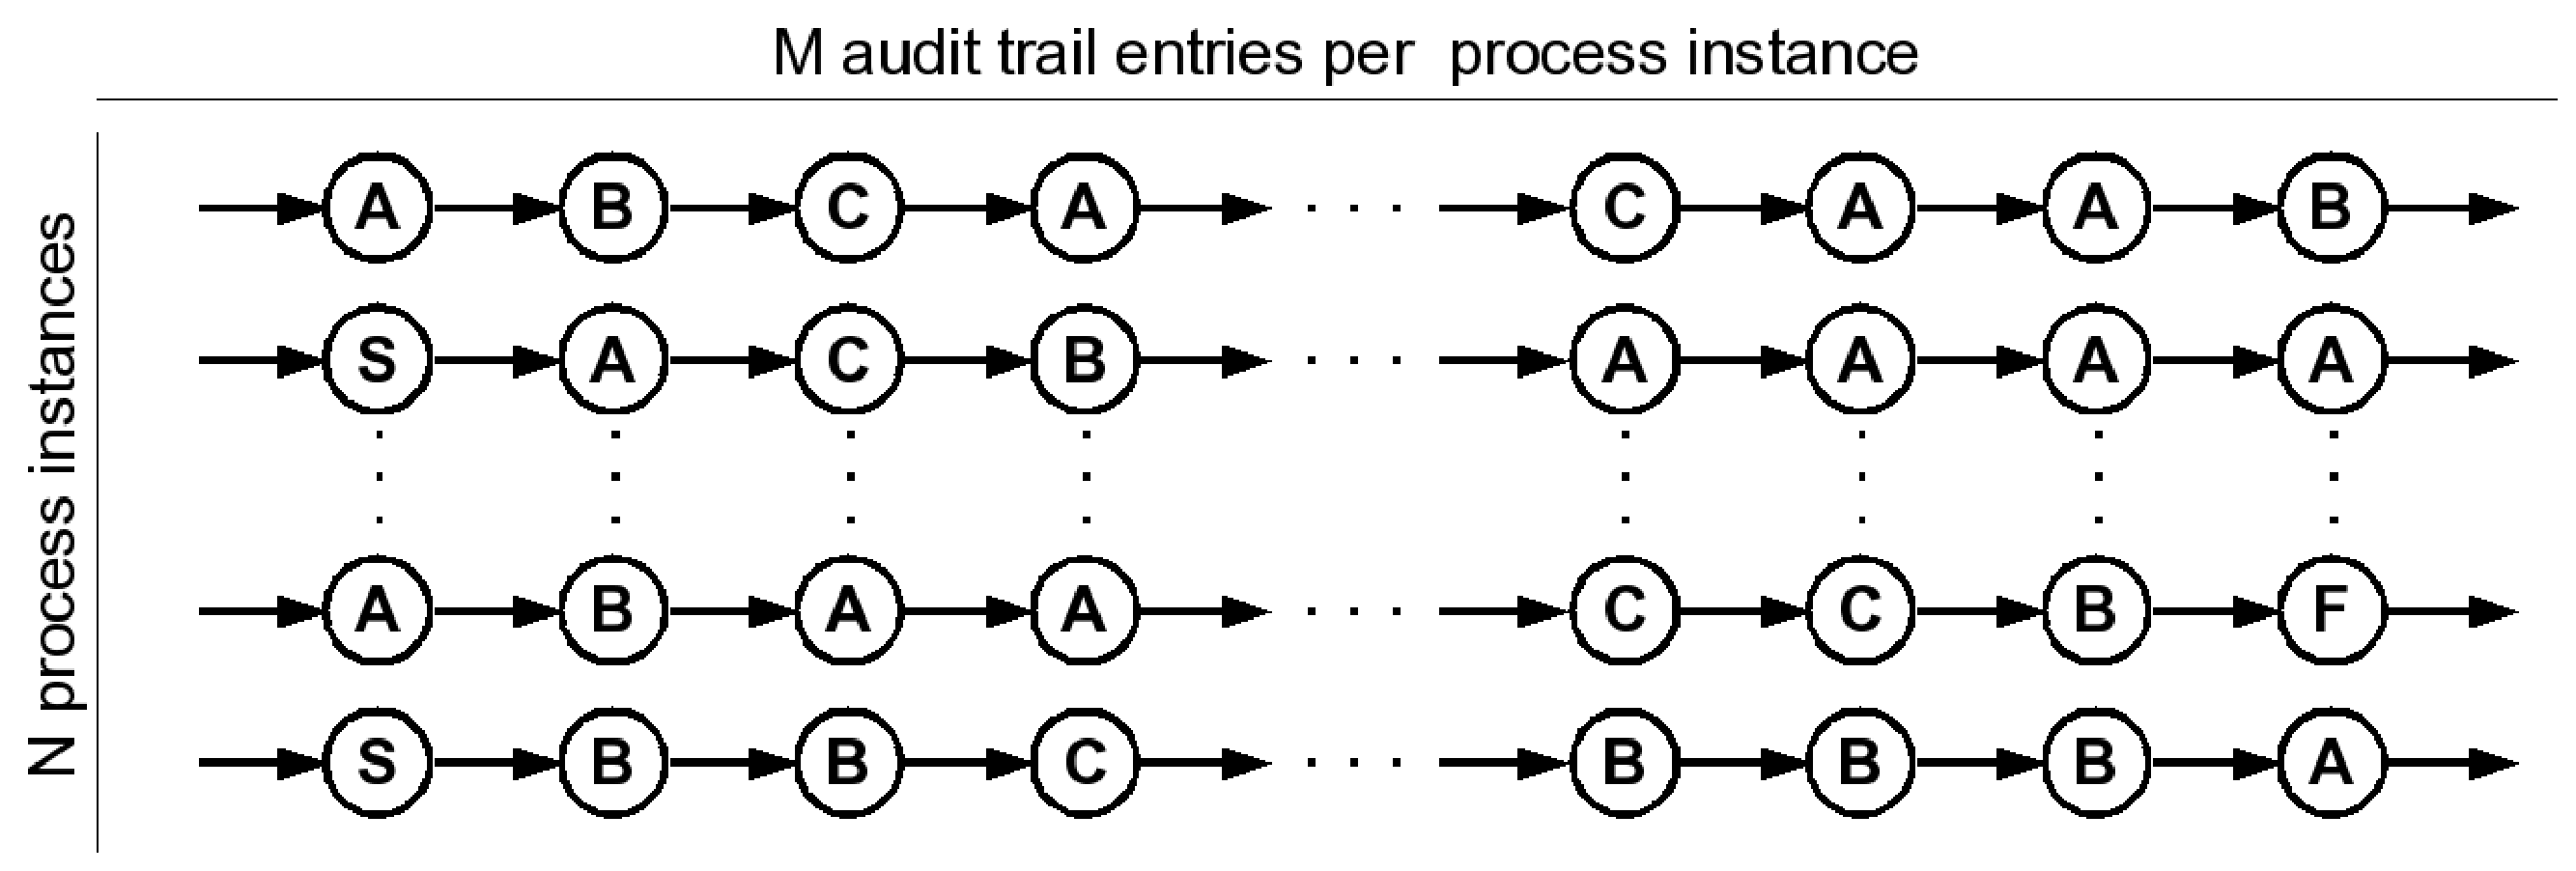
\includegraphics[scale=0.30]{diagrams/log-diagram.eps}
    \caption{A log}
    \label{language:log}
\end{figure}

In the language those date fields can be accessed by defining ( Subsection \ref{language:attribute}) attributes of the appropriate type (
number, set, string or date ) for the data fields. Later these attributes can
be used in logical expressions via comparisons ( Section \ref{language:comparison}). 

The value of these attributes depends on the "current" audit trail entry while
checking the log. A log is checked one process instance a time. Every process
instance is checked by inspecting the audit trail entries one for one from the
last till the first. The current audit trail entry is that audit trail entry
which is currently inspected by the checking algorithm.

The value of an attribute is computed by getting the value of the corresponding data field of
the current audit trail entry. If needed, this string value is parsed to the
appropriate type, thus in case the attribute is defined of type number or type
date it is parsed.

In the language you can use different sorts of logical expressions. First of
all, the "normal" propositional logic. This logic is about truth values only,
that is, an expression is true if the operator applied on the operands results
in true, otherwise it results false. The context of a propositional logic
expression is determined by the temporal operators. If no temporal operators
are used, a logical expression is about the first audit trail entry of a
process instance only.

Another sort of logic is the quantificational logic which you can use to
specify properties over all members of a set. Here again, the context of a
quantificational expression is determined by temporal operators.

The last kind of logical expressions are linear temporal logic expressions.
With these LTL operators you can specify properties about the current audit trail
entry, the next current trail entry given the current audit trail entry, any
audit trail entry given the current or all audit trail entries given the
current audit trail entry. The current audit trail entry is initial the first,
so by not using temporal operators, all logical expressions are about this
first current initial audit trail entry.

The temporal operators are the operators which gives you the possibility to
specify properties about a whole process instance, about all audit trail
entries of a process instance. You can specify temporal relations between
audit trail entries and so you change the context of the normal logical
expressions.

\subsection{A running Example}
\label{language:example}
\index{LTL Language!Running example}
\index{Examples!Description}

In this chapter a running example of a log existing of process
instances of persons doing different tasks is used. Every process instance has two
data fields: a name and a case number. For every audit trail entry minimal
three data fields are available: WorkflowModelElement, here called
\textit{task};
Originator, here called \textit{person} and Timestamp, here not used. Furthermore, all audit trail entries do have a EventType data
field, but the value is always \textit{complete} so this
field is not mentioned any more. 

\begin{figure}[H]
    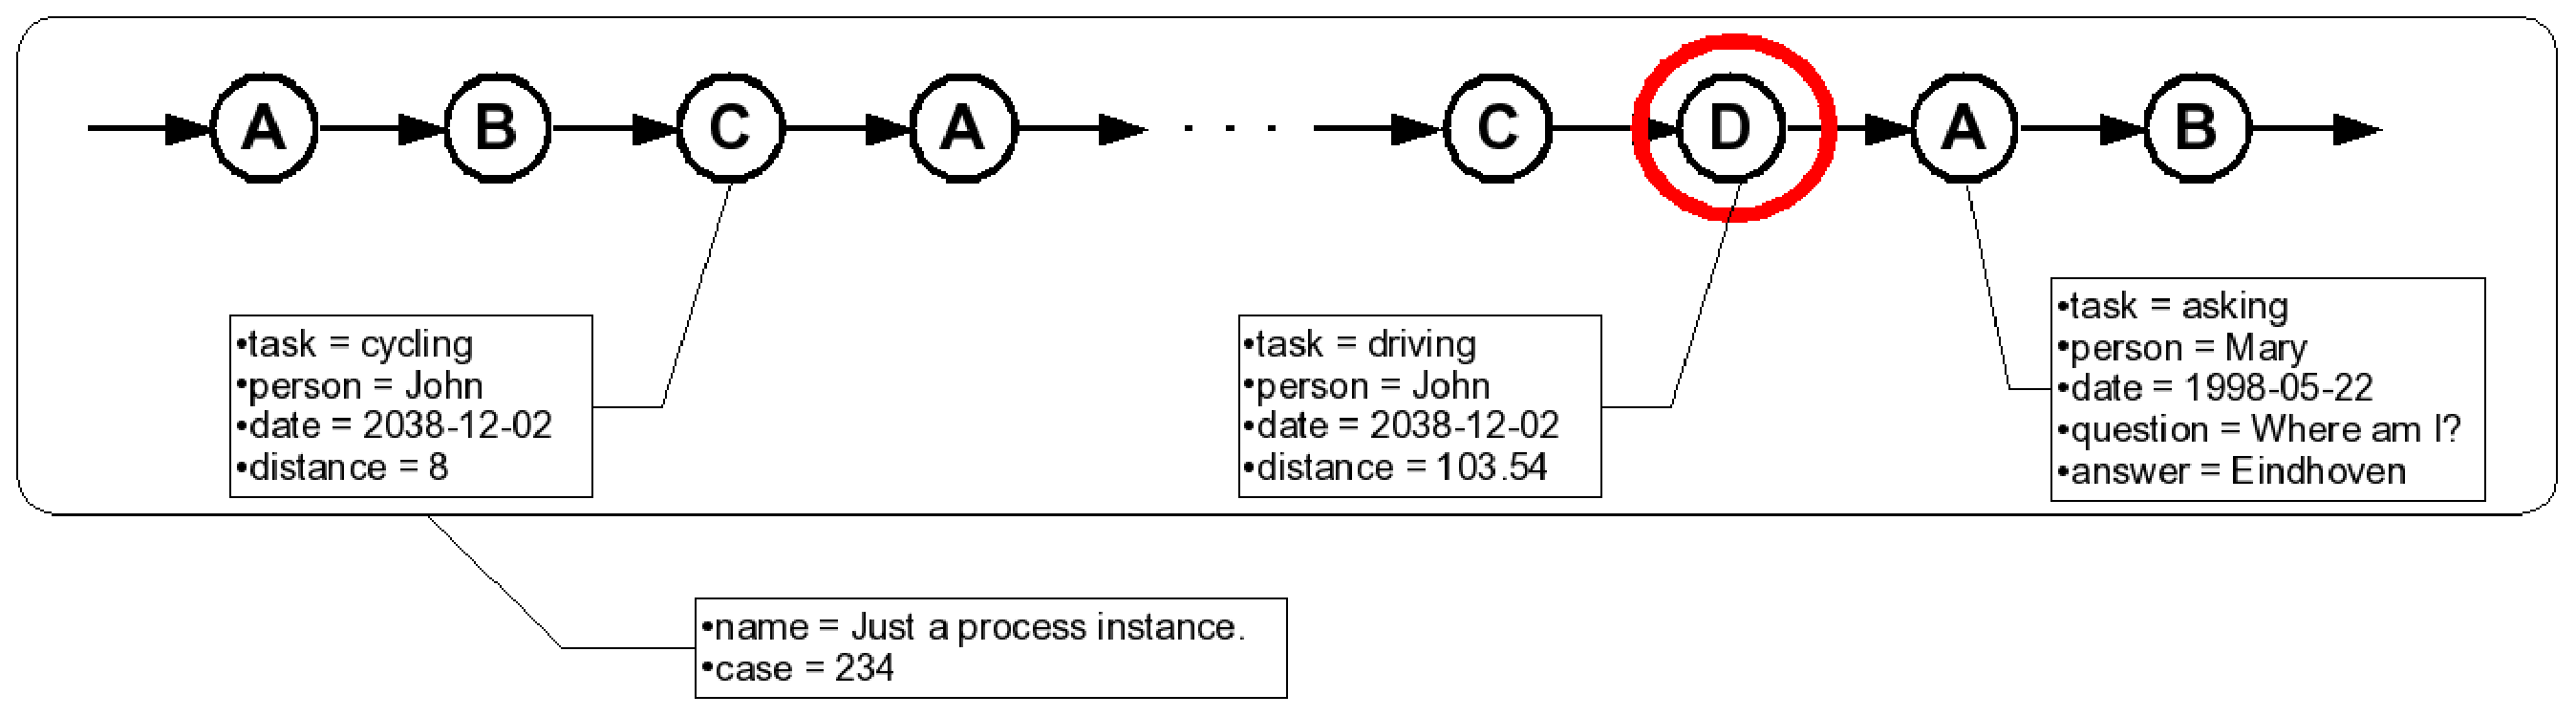
\includegraphics[scale=0.30]{diagrams/current-process-instance.eps}
    \caption{An example process instance}
    \label{language:pi01}
\end{figure}

Besides those standard data fields, audit trail entries can have extra data
fields depending on the task. In Figure \ref{language:pi01} you see a
visualization of one of such process instances of the example log. On the
figure you see the current process instance, that is the process instance for
which a property is computed. The current audit trail entry is the one with
the red circle ( or the grey circle) called \textbf{D}.

When new language elements are introduced they are explained by using this
figure. To be complete, for this running example there are two files added to
the manual: running.ltl and running.xml. The first file contains the ltl
properties specified this chapter and the second file contains a log to test
the properties specified in this chapter.

\section{Definitions and Comments}
\label{language:definitions}

An LTL Template file can consist of four different items: comments, attribute
definitions, renamings of those defined attributes and formula definitions.
Those items can be mixed in any order, but a definition can only be used if it
is already defined. Now the different items are described.

\subsection{Comments}
\label{language:comments}
\index{LTL Language!Comments}

Comments are the most simple elements of the language. A comment starts with a
\ltl{\#} and the rest of the line after the \ltl{\#}, including the \ltl{\#}
is skipped by the parser as comment.

It is a good practice to use comments in your LTL Template files to document your files in
such a manner that you and others can understand and adapt the file later on, also after
some time. It is very easy to create formulae, but to understand
them can be more difficult if the formulae becomes more complex, then comments can
be of great help.

\subsubsection{Examples}
\index{Examples!Comments}

We start our running example by creating some comment lines with some
information about the file:

\begin{ltlcode}
#######################################
# version  : 0.0
# date     : 01122004
# author   : HT de Beer
##
\end{ltlcode}

Of course comments at the start of a file only is not that useful. It is also
possible to use comments in definitions of formula, after attribute
definitions, the line before renamings, and so on. Later on in this chapter,
you will see examples of this.

\subsubsection{Parse errors}
\index{Error!Comments}

    No errors specified.

\subsection{Attribute Definitions}
\label{language:attribute}

Definitions of an attribute are more complex than writing comments, but it is easy
enough. An attribute definition starts with a keyword denoting the type of the
attribute. There are four types and thus four keywords: \ltl{number},
\ltl{set}, \ltl{string} and \ltl{date}.

After the type you give the name of the attribute. This name must be unique
and exists of two parts: a scope prefix and the name of the corresponding data
element in the workflow log. The scope prefix is either "\ltl{ate.}"
or "\ltl{pi.}" and denotes if the data element is an element of an audit trail
entry (\ltl{ate.}) or if the data element is an element of a process instance
(\ltl{pi}). So if a data element exists as well as a process instance element
and as an audit trail entry element, you can define both as an apart attribute
because the scope prefix results in two different names.

If you are not defining a date attribute, you are ready after putting a
semicolon. For a date attribute you should give the \ltl{:=} keyword followed
by a date pattern, and finally a semicolon too. Hereafter the different types
are described:

\begin{itemize}
    \item \ltl{number}\\
    \index{LTL Language!Defining attributes!Number}
    \index{Defining attributes!Number}
    The first type of attribute you can define is the \ltl{number} attribute. A
    number attribute can contain values that can be parsed as integers or floating
    point numbers. internally both integers and floating point numbers are
    parsed to floating point numbers only. Examples are: \ltl{12},
    \ltl{12.34}, \ltl{12.34e5}, \ltl{9E-23} and \ltl{-123444}.

    You define a number attribute for data element \textit{data-element} as follows:
    \ltl{number pi.data-element;} or \ltl{number ate.data-element;}, depending
    on the scope of the data element.

    \item \ltl{string}\\
    \index{LTL Language!Defining attributes!String}
    \index{Defining attributes!String}
    Attributes of type string are attributes which contain string values. Because
    in the log itself all data elements are strings, string attributes can
    be used for all data elements. No extra parsing is needed from the data
    element to an attribute. But when you want to use special properties of dates,
    numbers or sets, it is a good idea to define data elements of the respectively
    type. For the string type, a special regular expression operator is
    available ( Subsection \ref{language:regexp} ).

    You define a string attribute for data element \textit{data-element} as
    follows: \ltl{string pi.data-element;} or \ltl{string ate.data-element;},
    depending on the scope of the data element.

    \item \ltl{set}\\
    \index{LTL Language!Defining attributes!String}
    \index{Defining attributes!Set}
    The set type is used for quantification, because quantification can only be used on set type
    attributes. For every set attribute a real set containing all the
    unique values of this data element of all process instances and all audit
    trail entries is created. An extra set operator is the \ltl{in} operator
    ( Subsection \ref{language:in} ).
    
    You define a set attribute for data element \textit{data-element} as
    follows: \ltl{set pi.data-element;} or \ltl{set ate.data-element;},
    depending on the scope of the data element.

    \item \ltl{date}\\
    \index{LTL Language!Defining attributes!Date}
    \index{Defining attributes!Date}
    The last type is the date type. It can be used to access data
    elements containing date strings. Because there are many forms in which a
    date can be described, a special string, the date pattern is added to the
    date type attribute definition. The date pattern is afterwards used
    to create a SimpleDateFormat object of the Java
    programming language. The format of date patterns allowed is described at
    http://\-java.sun.com/\-j2se/\-1.4.2/\-docs/\-api/\-java/\-text/\-SimpleDateFormat.html,
    a web page containing information about the SimpleDateFormat class.

    For now we give a short description on how to create a date pattern, for a
    full explanation, read the web page mentioned earlier. In short, a date
    pattern exists of characters with special meaning. If you want to put
    characters themselves in a data pattern, use a "'" to enclose them. Now a
    table with some date characters are given. This list is not complete,
    therefor again, have a look at the web site mentioned earlier.

    \begin{tabular}{ll}
	y & year\\
	M & month in year\\
	w & week in year\\
	W & week in month\\
	D & day in year\\
	d & day in month\\
	E & day in week\\
	H & hour in day (0-23)\\
	k & hour in day (1-23)\\
	m & minute in hour\\
	s & second in minute\\
	S & millisecond\\
    \end{tabular}

    With these date characters, you now can build date patterns, like:
    \begin{itemize}
	\item \textit{yyyy-MM-dd} : thus strings of the form 2006-12-09.
	\item \textit{'date='ddMMyy} : strings like date=230907.
	\item \textit{HH:mm} : strings denoting time like 12:45.
    \end{itemize}

    You define a date attribute for data element \textit{data-element} and
    date pattern \textit{"date-pattern"} as
    follows: \ltl{date pi.data-element := "data-pattern";} or \ltl{date
    ate.data-element := "date-pattern";},
    depending on the scope of the data element.
\end{itemize}

An attribute can only be defined and used if there is a corresponding data
element. All data elements you want to query about should be defined as
an attribute, also the standard data fields like WorkflowModelElement,
EventType, Timestamp and Originator. That these elements are treated separate
from the other data elements in the logs, does not mean they are treated
special in the LTL Checker and LTL Language. In fact, in the LTL Language all
data elements, the standard ones too, are treated the same.

\subsubsection{Examples}
\index{Examples!Defining Attributes}
\index{Defining attributes!Examples}

Back to our running example of figure \ref{language:pi01}. As you can see in
this figure a number of attributes are available in the log. In this example
we define all the attributes: ate.WorkflowModelElement, ate.Originator,
ate.dob, ate.distance, ate.question, ate.answer, pi.name and pi.case.

\begin{ltlcode}
#######################################
# version  : 0.1
# date     : 01122004
# author   : HT de Beer
##

## 
# Defining attributes:
##
set ate.WorkflowModelElement;
set ate.Originator;
date ate.dob := "yyyy-MM-dd"; # Date of birth: dates have the format 'year-month-day'.
number ate.distance;
string ate.question;
string ate.answer;
string pi.name;
number pi.case;
\end{ltlcode}

\subsubsection{Parse errors}
\index{Error!Defining attributes}
\index{Defining attributes!Parse errors}

\begin{itemize}
    \item \textit{Identifier is already defined} 
    
    Occurs when you tries to define an
    attribute with the same name as another earlier defined attribute.    
\end{itemize}

\subsection{Renaming of defined Attributes}
\label{language:renaming}
\index{LTL Language!Renamings}
\index{Renamings}

A renaming is exactly what it says: a renaming. In this case you can rename a
defined attribute, which must be the name of the data element prefixed with
either "pi." or "ate.", to a shorter, more readable or understandable
alternative. In fact, you can define as many alternatives as you want, as long
as every alternative has an unique name.

\index{LTL Language!Name}\label{language:name}
Of course, as is usual in programming languages, a name can not be equal to
one of the keywords. Thus \ltl{as}, \ltl{ate}, \ltl{date}, \ltl{exists},
\ltl{forall}, \ltl{formula}, \ltl{in}, \ltl{number}, \ltl{pi}, \ltl{rename}, \ltl{set},
\ltl{string}, \ltl{subformula} are not permitted as names for renamings and
formulae. Furthermore, a name starts with a letter and can consists of letters, digits, -, and \_. 

A renaming can be created by the keyword \ltl{rename} followed by the
attribute name, the keyword \ltl{as}, the new name and finally the semicolon,
as is the case for all definitions. Thus for attribute name \textit{old-name}
and new name \textit{new-name} you write a renaming as follows: \ltl{rename
old-name as new-name;}.

\subsubsection{Examples}
\index{Examples!Renamings}
\index{Renamings!Examples}

We now adapt our running example so that the defined attributes are named as
in figure \ref{language:pi01}. So ate.WorkflowModelElement is renamed as task,
ate.Originator as person and ate.dob as bdate. For the other attributes
we rename them to a new name without the scope prefix.

\begin{ltlcode}
#######################################
# version : 0.2
# date : 01122004
# author : HT de Beer
##

## 
# Defining attributes:
##
set ate.WorkflowModelElement;
set ate.Originator;
date ate.dob := "yyyy-MM-dd"; # dates have the format 'year-month-day'.
number ate.distance;
string ate.question;
string ate.answer;
string pi.name;
number pi.case;

##
# Renamings
##
rename ate.WorkflowModelElement as task;
rename ate.Originator as person;
rename ate.dob as bdate;
rename ate.distance as distance;
rename ate.question as question;
rename ate.answer as answer;
rename pi.name as name;
rename pi.case as case;
\end{ltlcode}

\subsubsection{Parse errors}
\index{Error!Renamings}
\index{Renamings!Parse errors}

\begin{itemize}

    \item \textit{Identifier is already defined.}
    
    The new name is already in use as another renaming or formula name.

    \item \textit{Identifier is not a defined attribute.}
    
    You try to rename a formula or a renaming, but that is not possible. You can only rename
    attributes. 

\end{itemize}

\subsection{Formula Definitions}
\label{language:formula}
\index{LTL Language!Formula definitions}
\index{Formulae}

Now you can define attributes and rename them to something more writable, you
can use those definitions to define formulae. There are two kinds of formulae:
formulae and sub formulae. Both are defined exactly the same but the
first keyword, respectively \ltl{formula} and \ltl{subformula}, is different. The
distinction is that sub formulae are not visible in the Template GUI ( Section \ref{plugingui:templategui} ), that is, they can not be called by the
user of the GUI. Formulae are the visible formulae, the formulae which the
user can select and check.

A formula or subformula is defined as follows: the keyword \ltl{formula} or
\ltl{subformula} followed by an unique name, a list of parameters between
parentheses (the list may be empty), the keyword \ltl{:=}, a description, the
actual formula and finally the well known semicolon. Thus: \ltl{formula
A\_formula\_name ( arg1: attr1, arg2: attr2 ) := \{ A description \} actual
formula doing something with the arguments ;}.

The different elements of a formula definition are now explained.

\subsubsection{The list of arguments of a formula}
\index{LTL Language!Formula definitions!List of arguments}
\index{Formulae!List of arguments}

The list of arguments is a comma separated list of so called local renamings,
that is a new unique name in the local context followed by a colon and the
attribute the new name is a local renaming for. The name of the local renaming can
not be the same as a name of an attribute, renaming or formula, but it can be
the same as an argument of another formula. 

Furthermore the attribute, comparable with types in programming languages, is
an already defined attribute ( or a renaming of an attribute ). Such a pair
\ltl{argument\_name : attribute\_name} denotes that the name of the argument
must be interpreted as a local renaming of the attribute. In expressions later
on in the formula definition, this name can be used as such ( but only on the
right hand side of an comparison, see Section \ref{language:comparison} ).

The list, as said before, may be empty, but the parenthesis are obligatory in
all cases, also if the list is empty.

\subsubsection{The description of a formula}
\index{LTL Language!Formula definitions!Description}
\index{Formulae!Description}

A description of a formula is the part of the formula definition in which you
can inform the user of your defined formulae what the meaning and the use of
the formula is. In the Template GUI ( see section \ref{plugingui:templategui} ) the
contents of the description are displayed in the description pane. Because the
description pane renders its content as HTML 3.2, you can use those HTML 3.2
tags to create a more elaborate description for the user.

In fact, it is recommend to use HTML 3.2 code in your description. But only
the contents of the body tag should be used because the rest of the HTML code
is supplied by the plugin itself. Furthermore it is advisable to create your
descriptions along the guidelines given below, just to create a consistent
view for the user. On the other hand, it is all up to you to do so or not. I
know programmers are lazy, so empty descriptions shall be used much. In
principle, there is nothing wrong with that, as long as you are writing the
formula definitions for your own. But once you write your formulae for an
(unknown) audience, use the description wisely.

A description is made out of braces where in between the contents of the
description are placed. The guidelines for writing a description:\\
\begin{enumerate}
    \item Start with the title, or name of the formula in between \textit{h2}
    tags.
    \item Divide your description into paragraphs using the \textit{p} tags.
    \item In the first paragraph you give a short description of the meaning
    of the formula in terms of the arguments.
    \item in the next paragraph, or, in case of a simple formula in the first,
    you list the arguments using an unordered list( using the \textit{ul} tag.
    Every item in the list (create a list item with the \textit{li} tag)
    starts with the name of the argument in bold (\textit{b} tag), followed by
    the meaning of the argument. Give then the attribute in italics
    (\textit{i} tag ) and the type of the attribute ( eventually in italics
    too). Then a recommendation of
    the value the user should give. For example a range or the pattern of the
    date pattern in case of a date attribute.
    \item Write now a more detailed description and or other remarks if
    needed.
\end{enumerate}

\subsubsection{The actual formula}

The actual formula is given in terms of propositional logic (section
\ref{language:proposition}), quantification (section
\ref{language:quantification}),
linear temporal logic ( Section \ref{language:ltl} ), comparisons ( Section
\ref{language:comparison} )  or (sub)formula calls ( Section
\ref{language:formulacalls} ). That is, the actual formula consists of correct
expressions ( in this language ) combined to bigger expressions by the operators in
this language.

\subsubsection{Examples}
\index{Examples!Formula definitions}
\index{Formulae!Examples}

For the running example we define now one formula, in which you see all
elements of a formula definition. Because till now you have not learned how to
write the actual formula, a very simple formula is defined. The description as
is given here is the only full description according to the guidelines you
will read in this manual, because the goal is to learn to write ltl formulae,
not to write good descriptions.

\begin{ltlcode}
#######################################
# version : 0.3
# ... 
# This part of the file is as in example version 0.2
# ...
##
# Formulae
##
formula eventually_task_A_is_done_by_person_P( A : task, P: person ):=
\{
  <h2>Does eventually P task A?</h2>

    <p>Is there a audit trail entry in a process instance in which person P
    does task A?</p>

    <p>
      <ul>
        <li><b>A</b> is a task, of attribute <i>ate.WorkflowModelElement</i>.
        For this argument fill in the task you want to check for.</li>
        <li><b>P</b> is a person, of attribute <i>ate.Originator</i>. Fill in
        the person you want to know if he or she perform task A.</li>
      </ul>
    </p>
\}
  <>( ( task == A /\bs person == P ) );
\end{ltlcode}

\subsubsection{Parse errors}
\index{Error!Formula definitions}
\index{Formulae!Parse errors}

\begin{itemize}

   \item  \textit{Identifier already defined.}
   
   The name if this formula is already a defined identifier, either of an
   attribute, a renaming or another (sub)formula.

   \item \textit{Identifier is already defined or used.}
   
   The identifier used as argument name is already used as argument name or as
   a global identifier, that is of an attribute, a renaming or a formulae.

   \item \textit{Identifier is not a defined attribute or renaming.}
   
   The identifier used as 'type' of an argument is not a defined attribute or
   a renaming, so it can not fulfill the role of an argument type.

\end{itemize}

\section{Formula calls}
\label{language:formulacalls}
\index{Formula call}

A defined formula can be called in the actual formula part of a definition of
another formula. Important by calling a formulae is that the formula you want to
call must already be defined, you apply the right number of arguments, and, of
course, of the right type. That is, an argument of type A must be applied with
a value of type A, either an attribute itself ( the same, modulo renaming) or
a literal of the same type as the attribute.

You call a formula by entering the name followed by a parameter list surrounded
by parenthesis, this list may be empty, according to the definition of the
formula to call.

The value of an argument in a call is bound at that place. With this feature,
you get the value of a data element of an attribute of the audit trail entry
that is current at the place the argument is used. If in the formula a
nexttime operator is used, the current audit trail entry becomes the next one,
but the value of the argument supplied to this formula stays the of the
current one. 

This "early" binding can be useful when using the nexttime operator
( Subsection \ref{language:nexttime} ), because then the current audit
trail entry becomes the next one ( if there is a next one of course ). With a
formula call, you can supply such nexttime operator with a value of a
attribute before the then current. So you can apply recursion of a sort. But
you will read more on this subject in the subsection about the nexttime
operator.

\subsubsection{Examples}
\index{Examples!Formula calls}
\index{Formula call!Examples}

Because our running example has only one formula defined yet, we call it here
in a new defined formula.

\begin{ltlcode}
#######################################
# version : 0.4
# ... 
# This part of the file is as in example version 0.2
# ...
##
# Formulae
##
formula eventually_task_A_is_done_by_person_P( A : task, P: person ):=
\{
  <h2>Does eventually P task A?</h2>

    <p>Is there a audit trail entry in a process instance in which person P
    does task A?</p>

    <p>
      <ul>
        <li><b>A</b> is a task, of attribute <i>ate.WorkflowModelElement</i>.
        For this argument fill in the task you want to check for.</li>
        <li><b>P</b> is a person, of attribute <i>ate.Originator</i>. Fill in
        the person you want to know if he or she perform task A.</li>
      </ul>
    </p>
\}
  <>( ( task == A /\bs person == P ) );

formula does_John_drive() := 
\{ Does John drive in a process instance? \}
  eventually_task_A_is_done_by_person_P( "driving", "John" );
\end{ltlcode}

\subsubsection{Parse errors}
\index{Error!Formula calls}
\index{Formula call!Parse errors}

\begin{itemize}
    \item \textit{Identifier is not a defined formula.}
    
You try to use a identifier of a attribute or renaming as a formula, and of
course, you can not call such a identifier as a formula.

    \item \textit{Defined number of parameters not equal the number of arguments applied
here.}

You try to call a formula with not enough parameters, or with to much
parameters. Of course, this would not work, so assure that the number of used
parameters equals the number of defined arguments.

    \item \textit{Identifier has not the right type.}
    
You try to use a identifier of an attribute or renaming or a local one with a
different type ( attribute) than defined in the formula definition. If at
place x in the argument list a argument of type A is defined, use a value of
type A on place x in the parameter list of the formula call.

    \item \textit{Identifier is not a local parameter in this context.}
    
You try to call the formula with a identifier that is unknown in the local
context, so it is not known as a defined attribute or renaming, and not as a
argument to the formula in which the call is written down.

    \item \textit{Unable to parse this as a date given definition \textit{xyz}}
    
You fill in a date string as parameter, but this string can not be parsed
according to the definition of the used attribute in the argument list of the
formula definition.

    \item \textit{Type mismatch.}
    
You try to use a string value on an argument of attribute with type number.

    \item \textit{Not expecting a integer.}
    
A integer is applied where no number is expected.

    \item \textit{Not expected a floating point number.}
    
A floating point number is applied where no number is expected.

\end{itemize}

\section{Comparisons}
\label{language:comparison}
\index{LTL Language!Comparisons}
\index{Comparisons}

The basis of formula definitions are the comparisons, that is the comparisons
of attributes, and thus data elements of process instances of audit trail
entries, with other values, which may be attributes too, but literals are also
possible. All attribute types have a number of "standard" comparisons common,
and some have their own extra comparisons. First are the standard ones
explained, then per type the literals and special comparison operators
are described. But
before that, the common form of a comparison is given.

\begin{figure}[H]
    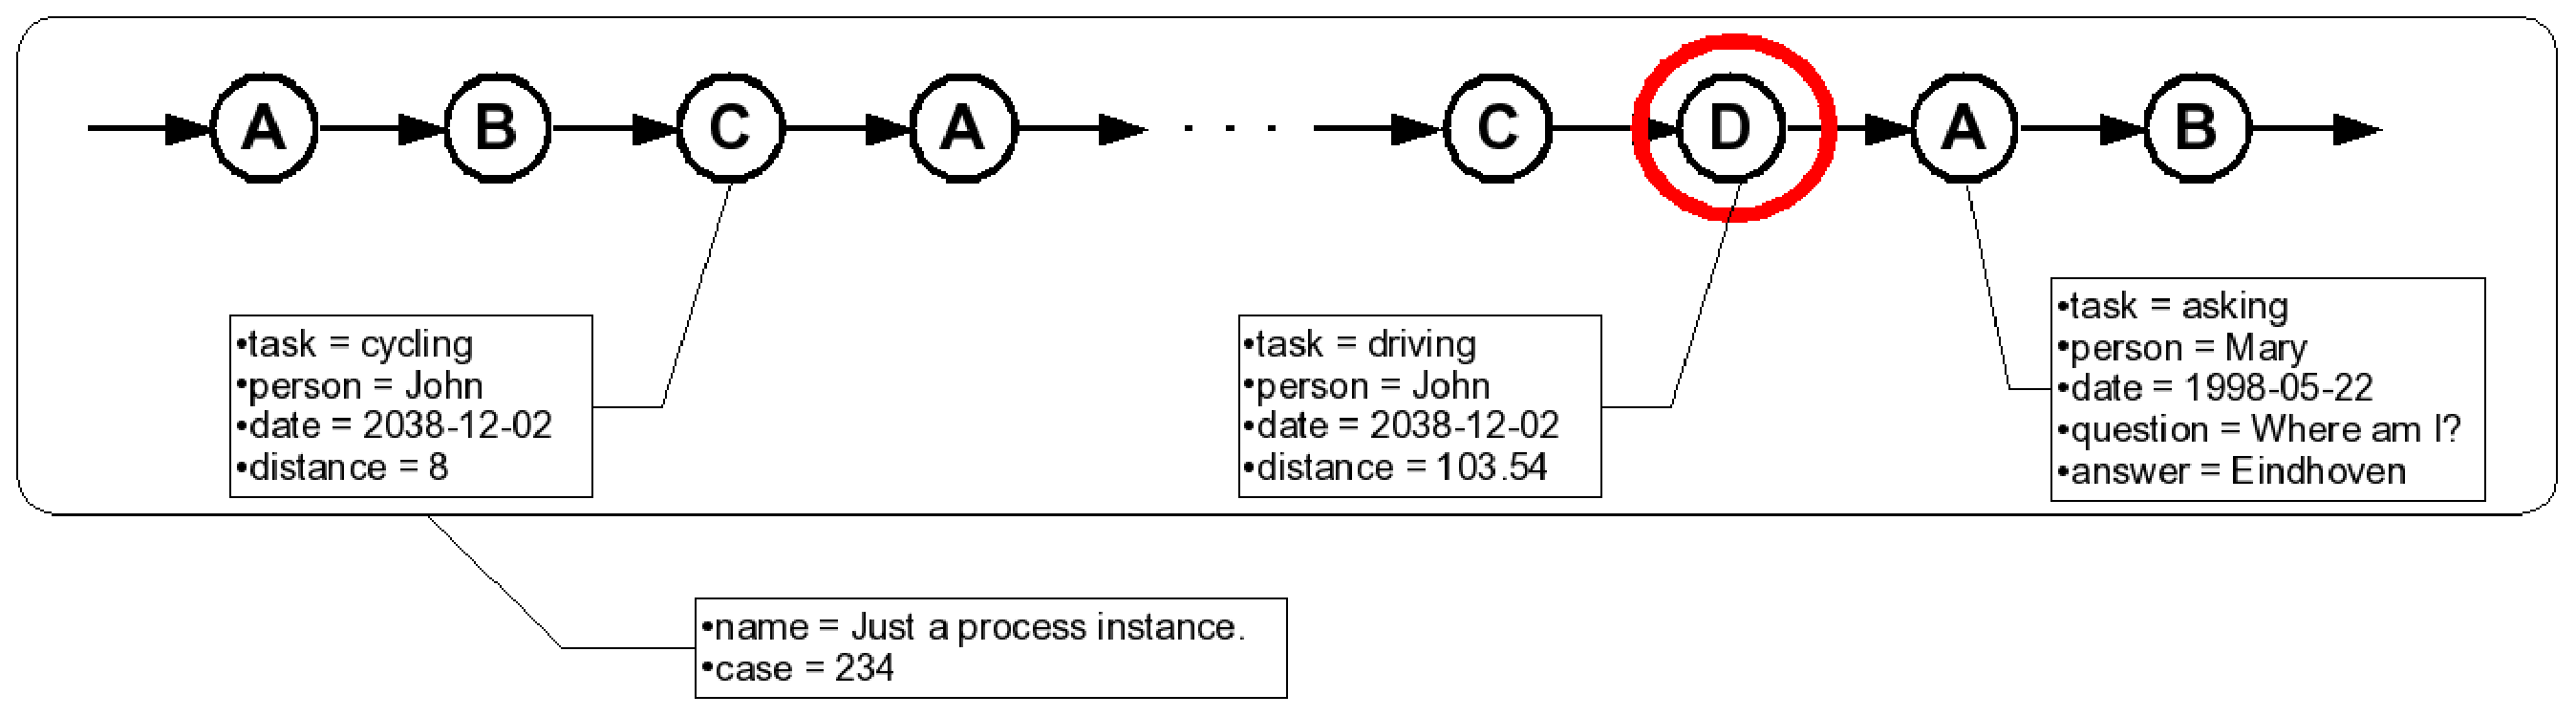
\includegraphics[scale=0.30]{diagrams/current-process-instance.eps}
    \caption{Again the example process instance}
    \label{language:pi02}
\end{figure}

A comparison exists of a left hand side attribute, thus no local argument,
with an operator and a right hand value. This right hand value is either a
literal, an attribute ( or renaming, or local argument) or a more complex
expression in case of number attributes.

A comparison results always false if in the current audit trail entry the left
hand side attribute ( and thus a eventually right hand side attribute too)
does not exist. In the running example a comparison of the form \ltl{answer ==
"..."} results in false because the current audit trail entry, D, has no
answer data element.

So if you use a data element which does not exist for all audit trail entries,
be aware of the strange or unexpected results formulae may result.

\subsection{Standard comparisons}

\subsubsection{\ltl{==}}

The first standard comparison is the well known equivalence or "is equal"
operator \ltl{==}. It compares the left hand side with the right hand side. Of
course it is true when both sides results in the same value given the current
audit trail entry ( and process instance). 

In the example situation of Figure
\ref{language:pi02} where the audit trail entry labeled 'D' is the current
audit trail entry, a comparison like \ltl{ task == "driving" } would result in
true, because task, referring to the ate.WorkflowModelElement and
corresponding data element has in the log the value "driving". 

If the comparison was \ltl{ task == "asking" } it would result in false,
because the data element WorkflowModelElement of the current audit trail entry
has value "driving".

\subsubsection{\ltl{!=}}

The "is not equal" operator \ltl{A != B} is equal to \ltl{!( A == B )} (
Subsubsection \ref{language:not} ), and is the
reverse of the \ltl{==} operator. So in the running example where D is the
current audit trail entry, \ltl{ task != "asking" } is now true and \ltl{ task
!= "driving" } false.

\subsubsection{\ltl{$<=$}}

The "lesser than or equal" operator is denoted as \ltl{$<=$} and does just what you
expect that it does. Especially for date and number attributes this operator
and the counterparts \ltl{$>=$}, \ltl{$<$} and \ltl{$>$} are useful. For
string and set attributes you can use them for properties about the
alfa numerical ordering of strings. 

In the example \ltl{ distance <= 200 } results in true in the current audit
trail entry there the distance is equal to $103.54$.

\subsubsection{$>=$}

The bigger than or equal operator is denoted as \ltl{$>=$} and does just what you
expect, as all the standard operators do.

\subsubsection{$<$}

The lesser than operator is denoted as \ltl{$<$}.

\subsubsection{$>$}

The bigger than is denoted as \ltl{$>$}.

\subsection{The string type operators and literals}
\index{LTL Language!String}

A string literal looks like most string literals in most programming
languages: two quotes in which between the contents of the string is written
down. In principle every character can be in the string, only quotes
themselves are not permitted because they close the literals. For example
\ltl{"Hello world!"} or \ltl{"980u908009ud0f098s0d8uf0u8sd0ff8us09d"} are both
correct strings. 

For strings there is an extra operator: the regular expression operator
\label{language:regexp}
\ltl{\~{}=}. This operator has as string literal a string which is interpreted
as a regular expression pattern. Internally the \textit{matches} method of the
Java String class is used, so if you want to know all the details of the
patterns have a look at
http://\-java.sun.com/\-j2se/\-1.4.2/\-docs/\-api/\-java/\-util/\-regex/\-Pattern.html\#sum.

Now follows a short introduction of regular expressions. With regular
expressions you can specify patterns of characters, using special regular
expression operators. 

\begin{tabular}{lll}
Operator & Meaning & Example \\
. & A arbritrary character & ma. : like may, mad, man, mau, ...\\
$\hat{}$ & The start of a line & \\
\$ & The end of a line & \\
regexp? & Zero or one time regexp & ma? : , ma\\
regexp+ & One or more times regexp & ma+ : ma, mama, mamama, ...\\
regexp* & Zero or more times regexp & ma* : , ma, mama, mamama, ...\\
regexp{x,y} & Between x and y times regexp & ma{1,2} : ma, mama\\
re1 $|$ re2 & re1 or re2 & ma $|$ pa : pa or ma\\
re1re2 & re1 followed by re2 & mapa : mapa, mamapa, mamamapa, ...\\
(re1) & Group re1 & ma(pa)?ma : mama, mapama\\
$[$x-y$]$ & Element of x...y & $[$1-9$][$0-9$]$+ : a number like 9, 83, 3859, ...\\
$[$abc$]$ & Element of a b c & $[$dmy$][$1-9$]$ : d3, y5, m5, m3, ...\\
\end{tabular}

With the building blocks given in this table you can construct more elaborate
regular expressions, and more operators are available. To conclude this very
short introduction on regular expressions, some examples:\\
\begin{itemize}
\item \textit{.*word.*} Search for strings with 'word' in it, like this
sentence.
\item \textit{ID[0-9]\{5,5\}} Search for strings starting with ID and followed
by five digits. ID98324, ID12347, etc.
\item \textit{a*b*} Search for sequences of n a's, followed by m b's, like
aabb, abbbbbbbb, aaaaaaaabbbb, etc.
\item \textit{yes$|$Yes$|$y$|$Y} Search for different ways to express yes.
\end{itemize}

\subsection{The set type operators and literals}
\index{LTL Language!Set}

The set literals are exactly the same as string literals. That is easy
explained: the sets exists of just strings. Furthermore, the standard
operators can be seen as a cast to strings before using them, so you can test
an individual value of the set to another value. Sets are used for
quantification, and therefor it is an apart type.

Nevertheless a special set operator is defined: the \ltl{in} operator.
\label{language:in}It
tests if the left hand side attribute is in a by the user given set. It is
of the form attribute, the \ltl{in} keyword, and a list of strings, separated
by comma's between
"[" and "]". Because the language does not enforce the list to test for
duplicates in the set, it can be a multiset or bag too. In fact, internally it is transformed to
a set, but for you as user of the \ltl{in} operator, it is a bag. In the
running example a expression could be \ltl{ person in [ "John", "Mary",
"Angilbert"]}, that is, test whether the person of the current audit trail
entry is either "John", "Mary", or "Angilbert". In this case, it results true
because in the current audit trail entry 'D' the person is "John".

\subsection{The date type literals}
\index{LTL Language!Date}

The type date has no extra operators, but the literals themselves are more
powerful. In principle they are string literals too, but are interpreted with
the by the date attribute on the left hand side of the operator associated
date pattern. Those date patterns are explained before ( Subsection
\ref{language:attribute} ).

\subsection{The number type literals and expressions}
\index{LTL Language!Number}

On the type number there are no extra comparison operators defined, but more
complex numerical expressions are possible. Number literals are either
integers or floating point numbers. That is, just digits, or digits with a
period and eventually an exponent ( for example \ltl{123}, \ltl{0.4500988} or
\ltl{314.9067E234} ).

The numerical operators are the well known ones: \ltl{-}, \ltl{+}, \ltl{*} and
\ltl{/}. The unary operator \ltl{-} is used as \ltl{- value } and the binary
ones as \ltl{( value \textit{op} value )}. The placing of parenthesis are a little
bit strange and strict, but they are strict too by the logical operators.
Values can be either numerical expressions, number attributes ( or renamings or arguments ) or
number literals.

\subsection{Examples}
\index{Examples!Comparisons}
\index{Comparisons!Examples}

To the running example some helping formulae are defined with using some
comparison operators and literals. Because those comparisons are combined to
larger expressions with logical operators ( Section \ref{language:proposition}
), those logical operators are used although the meaning may not be completely
clear yet.

\begin{ltlcode}
#######################################
# version : 0.5
# ... 
# This part of the file is as in example version 0.4
# ...

subformula has_Answer() := \{
 If the task is asking, then there is a answer not equal to the empty string.
 This formula results in true for all task other than asking and for those
 task equal to asking with a non empty answer.
\}
  ( task == "asking" -> answer != "");

subformula distance_between( lbound: distance, ubound: distance ) := \{
 The distance of the current audit trail entry lies between the lower bound
 and the upper bound. \}
  ( distance >= lbound /\ distance <= ubound );

subformula reasonable_distance() := \{
 If the task is cycling, the distance must be between 0 and 65, if the task
 is driving is must be between 0 and 300, if the task is flying, the distance
 must be between 150 and 1340. \}
  (    ( task == "cycling" -> distance_between( 0, 65 )     ) /\bs
    (  ( task == "driving" -> distance_between( 0, 300 )    ) /\bs
       ( task == "flying"  -> distance_between( 150, 1340 ) )
    )
  );

subformula permitted_to_drive() := \{
 A person is permitted to drive if he or she is born before 2004-6-01. \}
  bdate < "2004-06-01";

subformula a_important_case() := \{
 Case is important if the word 'important' is used in the name. \}
  name ~= ".*important.*";  
\end{ltlcode}

\subsection{Parse errors}
\index{Error!Comparisons}
\index{Comparisons!Parse errors}

\begin{itemize}

\item \textit{Identifier is not of type string.}

This error is shown if you try to use the regular expression operator
\ltl{\~{}=} on attributes not of type string.

\item \textit{Identifier is not of type set.}

This error is shown if you try the \ltl{in} operator with attributes not of
type set.

\item \textit{Expected value of type number.}

You have used the special numerical operators with values or attributes (
which are more or less values too) not of type number.

\item \textit{Unable to parse this as a date given definition . . . . .}

Shown when you specify a date literal which is not parseble with the pattern
specified by the associated left hand side date attribute.

\item \textit{Expected a string.}

You use a left hand side attribute of type string, but the value you specified
can not be parsed as such.

\item \textit{Identifier not defined.}

You try to use an attribute or renaming as a value which is not defined before
use, hence this error.

\item \textit{Type mismatch}

The left hand side attribute and right hand side value does not match types.

\end{itemize}

\section{Propositional Logic}
\label{language:proposition}
\index{LTL Language!Propositional logic}
\index{Propositional logic}

Now the comparisons and literals are explained, the basis for the
propositional logic is laid because the atoms of the propositional logic in
the LTL language are those comparisons. Furthermore, properly defined formulae
exists of atoms too, so they can be seen themselves as behaving like atoms,
that is, resulting in true or false. Let A and B correct atoms or formulae.
They are used to combine them with logical operators to larger expressions.

\begin{figure}[H]
    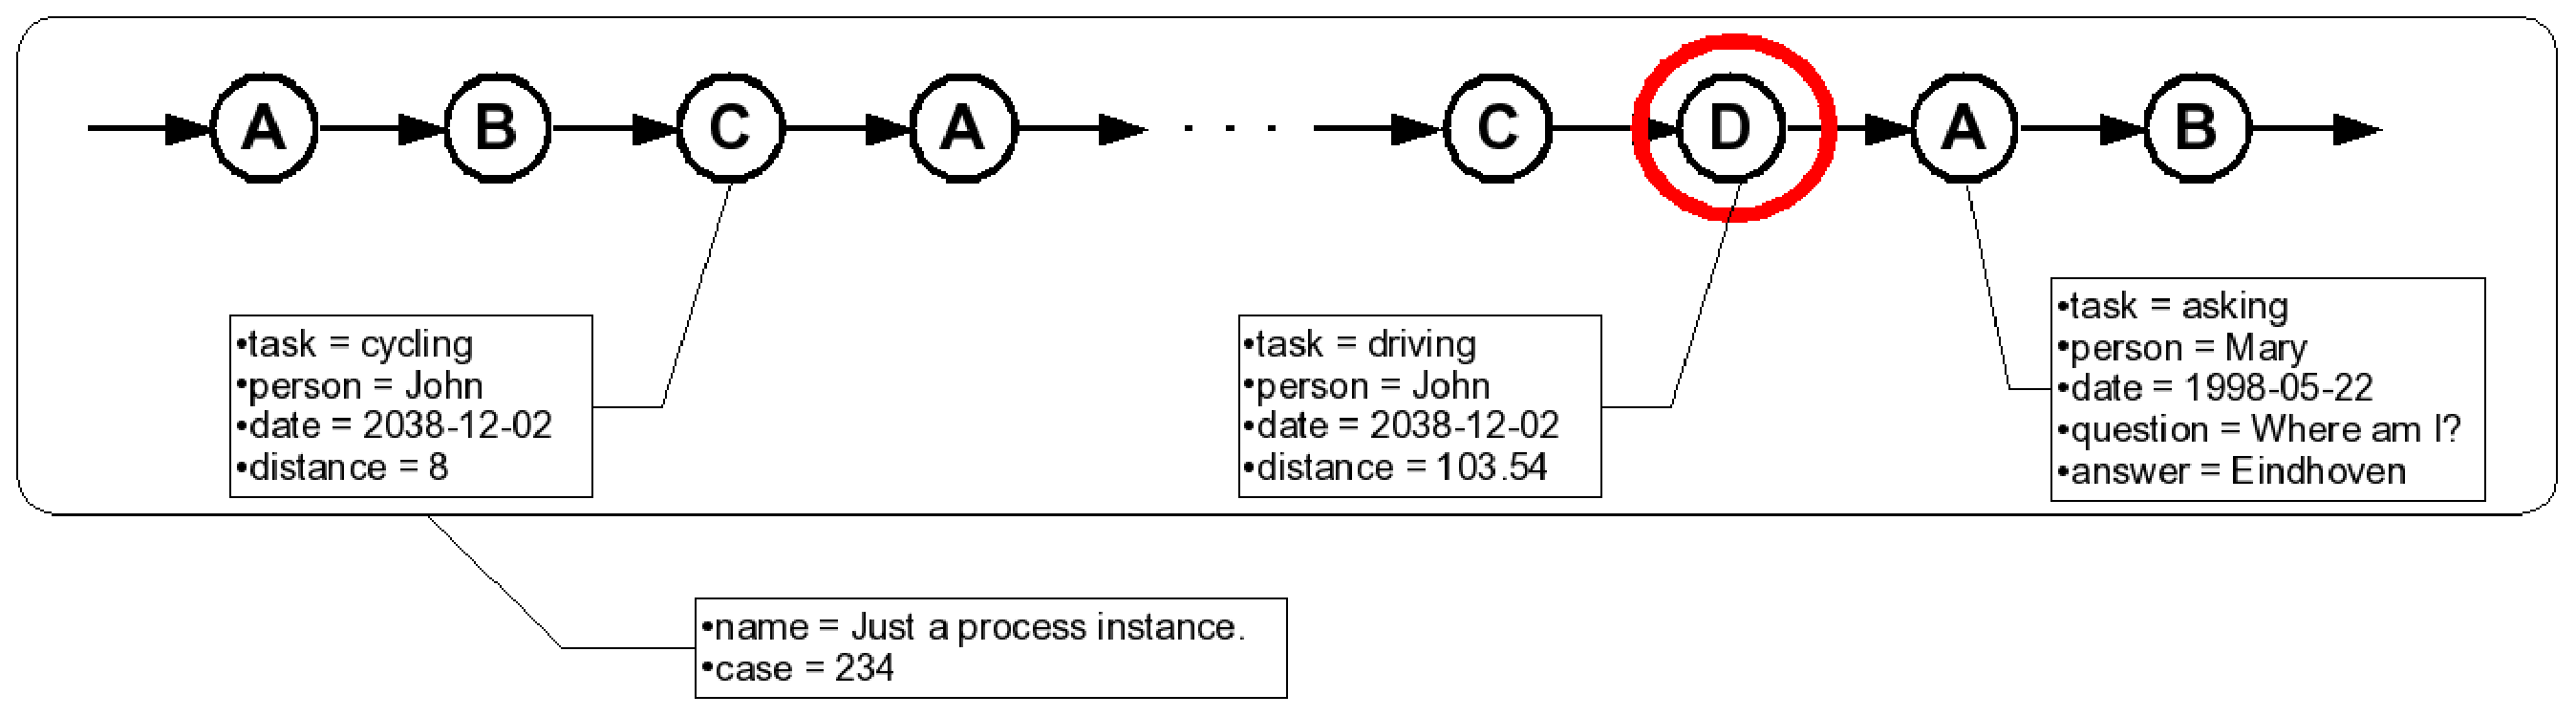
\includegraphics[scale=0.30]{diagrams/current-process-instance.eps}
    \caption{Again the example process instance}
    \label{language:pi03}
\end{figure}

The explanation of the logical operators is done with the use of the running
example where the current audit trail entry is as it was before: D ( Figure
\ref{language:pi03} ).

\subsection{Not}
\label{language:not}
\index{LTL Language!Propositional logic!Not}
\index{Propositional logic!Not}

The proposition \ltl{!( A )} is true if and only if A itself is false. In a
table:\\
\begin{tabular}{c|c}
A & \ltl{!( A )}\\\hline
0 & 1\\
1 & 0\\
\end{tabular}

As an example let A be \ltl{answer == "Eindhoven"}. Now A is false, because
there is no answer data element in the current audit trail entry D, so \ltl{!(
answer == "Eindhoven")} is true. But the reverse holds too: let A be
\ltl{distance < 1000}, with the distance equal to $103.54$, you will see
easily that the expression \ltl{!( distance < 1000 )} results in false.

\subsection{And}
\label{language:and}
\index{LTL Language!Propositional logic!And}
\index{Propositional logic!And}

The proposition \ltl{( A /\bs B )} is true if and only if A and B are
together true. In a table:\\
\begin{tabular}{c|c|c}
A & B & \ltl{( A /\bs B)}\\\hline
0 & 0 & 0\\
0 & 1 & 0\\
1 & 0 & 0\\
1 & 1 & 1\\
\end{tabular}

A simple example is \ltl{ ( task == "driving" /\bs person == "John" )} which
is true. In the next audit trail entry, this would be false, both the task and
the person are different, namely asking and Mary.

\subsection{Or}
\label{language:or}
\index{LTL Language!Propositional logic!Or}
\index{Propositional logic!Or}

The proposition \ltl{( A \bs/ B )} is true if and only if A or B is
true ( if both are true it is correct too, of course ). In a table:\\
\begin{tabular}{c|c|c}
A & B & \ltl{( A \bs/ B)}\\\hline
0 & 0 & 0\\
0 & 1 & 1\\
1 & 0 & 1\\
1 & 1 & 1\\
\end{tabular}

If the and operator in the last example is replaced with an or operator, it
stays true in the current audit trail entry. It is even true in the third
audit trail entry, where the person is John too.

\subsection{Implication}
\label{language:implication}
\index{LTL Language!Propositional logic!Implication}
\index{Propositional logic!Implication}

The proposition \ltl{( A -$>$ B )} is false if and only if A is true and B is
false.  But be aware, the arrow denotes a logical value, not a causal relation
 or a time relation at all. When one wants to state something about relations in
 time, thus that if A holds next time should hold B, use the nexttime operator
 \ltl{\_O}. In a table:\\
\begin{tabular}{c|c|c}
A & B & \ltl{( A -$>$ B)}\\\hline
0 & 0 & 1\\
0 & 1 & 1\\
1 & 0 & 0\\
1 & 1 & 1\\
\end{tabular}

If a property is only important if another property hold, for example a
(birth) date
must be before "2000-06-05" when the task is driving. That is, a person must
be old enough to be permitted to drive a car, the implication is useful:
\ltl{( task == "driving" -$>$ bdate < "2000-06-05" )}. But if driving does not
hold, the property with the implication is true. If you want to ensure that
the task is driving and if the task is driving then the date is lesser than
some value, use the and operator: \ltl{( task == driving /\bs bdate <
"2000-06-05" )}.

\subsection{Bi-implication}
\label{language:biimplication}
\index{LTL Language!Propositional logic!Bi-implication}
\index{Propositional logic!Bi-implication}

The proposition \ltl{( A $<$-$>$ B )} is true if and only if A and B have the
same value. This operator is also known as equivalence. In a table:\\
\begin{tabular}{c|c|c}
A & B & \ltl{( A $<$-$>$ B)}\\\hline
0 & 0 & 1\\
0 & 1 & 0\\
1 & 0 & 0\\
1 & 1 & 1\\
\end{tabular}

As a example state that a non empty question is equivalent with a non empty
answer. Thus, if both are not in the current audit trail entry, or both are
empty, then it is true. If one of the data elements answer or question is
empty or does not exist, then it is false. If both does exist and are not
empty, it is true too. \ltl{( question != "" $<$-$>$ answer != "" )}. This
is true in the current and the next state too.

\subsection{Examples}
\index{Examples!Propositional logic}
\index{Propositional logic!Examples}

In our running example we have already used some propositional logic
operators, in the next two sections, the logical operators are also used, so
for now no addition to the running example. 

\subsection{Parse errors}
\index{Error!Propositional logic}
\index{Propositional logic!Parse errors}

    No errors specified.

\section{Quantificational Logic}
\label{language:quantification}
\index{LTL Language!Quantification}
\index{Quantification}

Quantification in this language exists of the universal (\ltl{forall}) and
existentional (\ltl{exists}) quantor. The meaning of quantification is in this context not that
clear, or to say it otherwise, formulae defined in this language can be seen
as universal quantification over all process instances of the log.

Furthermore the LTL operators always (\ltl{[]}) and eventually (\ltl{$<>$}) can
be compared with respectively the universal and the existentional quantor
because if there exists an audit trail entry with
property A, then eventually holds A. And if always holds A, then for all audit
trail entries hold A. But quantification is not directly about audit trail
entries, but over sets, so the comparison between those LTL operators and
quantification is not complete, there are properties which can not be
specified with the LTL operators, but can with the quantors, and vice versa. 

On the other hand there is a drawback by using quantification, it is very costly because quantification over a set
S with property A results in a property of length $|$S$|$ times the length of A. So it is
advisable to try to use the LTL operators in stead of the quantors when
possible. But, as said before, quantification is sometimes needed, mostly to say something about all
elements of a set. If one wants to ask about one specific instance of a set,
use the LTL operators.

The standard data elements of an audit trail entry, WorkflowModelElement,
EventType and Originator are the most likely candidates for quantification,
and thus for being a set attribute. But all data elements can be sets and
therefor used for quantification, so Timestamp or distance too. But then, those attributes are sets, and the value
of the element is a string rather than a date or a number.

\subsection{Universal Quantor}
\label{language:forall}
\index{LTL Language!Quantification}
\index{Quantification}

The universal quantification computes if a property A holds for every element
in a set S. That is the property $\forall_{s \in S}(A_s)$. An universal
quantification is written as follows: \ltl{forall [ i:
SetAttribute $|$ A$_i$ ]}. With i: SetAttribute a local renaming i for
attribute SetAttribute of type set. The property to check for all i is then A.
If A holds for all i, this quantification is true.

\subsection{Existentional Quantor}
\label{language:exists}
\index{LTL Language!Quantification}
\index{Quantification}

The existentional quantification computes if a property A holds for any element
in a set S. That is the property $\exists_{s \in S}(A_s)$. An existentional
quantification is written as follows: \ltl{exists [ i:
SetAttribute $|$ A$_i$ ]}. With i: SetAttribute a local renaming i for
attribute SetAttribute of type set. The property to check for all i is then A.
If A holds for any i, this quantification is true.

\subsection{Examples}
\index{Examples!Quantification}

In the running example are now more complex properties specified using
quantification. For example a formula to test if there is a person doing two
different tasks. The universal quantification is used to specify the property
that all persons doing either moving or asking around, not both. Both
properties are about one process instance, and that for all process instances.

\begin{ltlcode}
#######################################
# version : 0.6
# ... 
# This part of the file is as in example version 0.5
# ...

subformula P_does_A-A_not_B( P: person, A: task, B: task ) := \{ 
 Compute if person P does task A, which is not equal to B.\}
  <>( ( task == A /\bs ( task != B /\bs person == P ) ) );

formula exists_person_doing_two_different_tasks() := \{
 Is there a person doing two different tasks?\}
  exists[ p: person   |
    exists[ t: task   |
      exists[ u: task |
        (  P_does_A-A_not_B( p, t, u) /\bs
           P_does_A-A_not_B( p, u, t)) 
      ]
    ]
  ];

subformula moving( P: person ) := \{
 Compute if person P is moving. \}
  <>( ( person == P /\bs
        (   task == "driving" \bs/ 
          ( task == "cycling" \bs/
            task == "flying"
          )
        )
    ) );

subformula asking( P: person ) := \{
 Compute if person P is asking. \}
  <>( ( person == P /\bs task == "asking" ) );

formula moving_or_asking() := \{
 All persons are either moving or asking around.\}
  forall[ p: person |
    ( 
      ( moving( p ) /\bs !( asking( p ) ) ) \bs/
      ( !( moving( p ) ) /\bs asking( p ) )
    )
  ];
\end{ltlcode}

\subsection{Parse errors}
\index{Error!Quantification}

\begin{itemize}

\item \textit{Identifier already in use in the local context.}

You try to use a name for the dummy variable which is already used for
something else.

\item \textit{Identifier is not a defined attribute or renaming.}

The attribute you want quantify over is not defined.

\item \textit{Identifier has not type set.}

The attribute you want quantify over is not a set.

\end{itemize}

\section{Linear Temporal Logic}
\label{language:ltl}
\index{LTL Language!LTL}
\index{LTL}

The LTL language elements are the logical elements which express properties
about a sequence of audit trail entries of a process instance. So an LTL
property A is not a logical expression about the current audit trail entry,
but over the sequence of audit trail entries described by logic expressions
about the current audit trail entry. A and B are correct sub formulae as
described earlier.

\begin{figure}[H]
    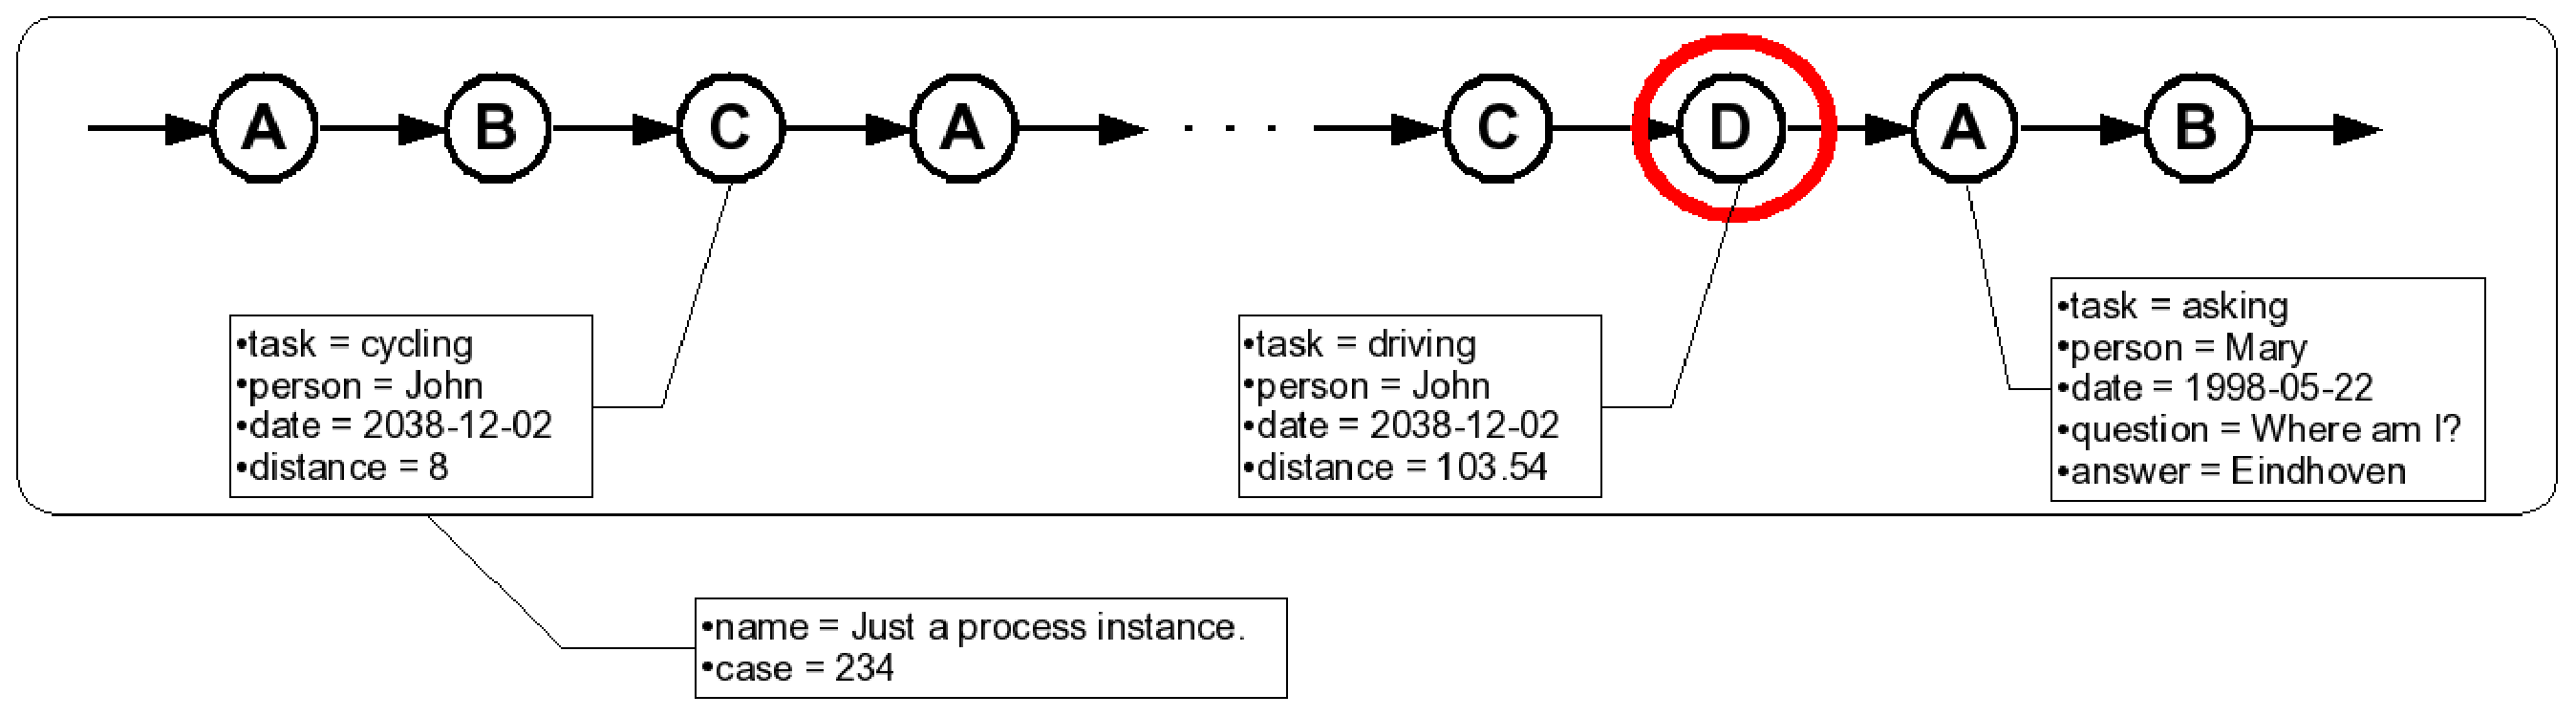
\includegraphics[scale=0.30]{diagrams/current-process-instance.eps}
    \caption{Again the example process instance}
    \label{language:pi04}
\end{figure}

Again the figure of the running example, now to explain the LTL operators.

\subsection{Nexttime}
\label{language:nexttime}
\index{LTL Language!LTL!Nexttime}
\index{LTL!Nexttime}

The nexttime operator is a very basic and simple operator. It express given a
current audit trail entry something about the next audit trail entry in the
sequence of audit trail entries in the current process instance. So you can
express more or less properties about subsequent states which have occurred.


The nexttime operator is an unary operator written as \ltl{\_O( A )}.
In the Figure \ref{language:pi04}, where the current audit trail entry is D,
\ltl{\_O( person == "Mary" )} is true because in the next audit trail entry,
with name A, the person is Mary. If the current audit trail entry was not D
but the C before it, then \ltl{\_O(\_O( person == "Mary" ) )} was true too.
You see, the nexttime operator can be used repeatedly to express some
property about a specific audit trail entry given the current.

Use this nexttime operator to express recursion about states. Then, with the always
operator (see below) you can check if a property A holds for all states of a
process instance. Remark that A never hold in the last state, so to apply such
recursion, identify the last state, so that always nexttime A holds or it is
the last state. Combined with a formula call, you can use values of other
states in the current comparisons.

For finalization, it is recommended to use an end formula: 
\begin{ltlcode}
subformula end() := \{ 
 Only in the last state holds that in the next state a
 WorkflowModelElement is not equal itself ( for other elements the same of
 course) because in the next audit trail entry of the last state all
 comparisons are false, the data elements does obviously not exist.\}
  !( _O( ate.WorkflowModelElement == ate.WorkflowModelElement ));
\end{ltlcode} 
  
  Using this end formula, it is also possible to specify properties relative to the last
 state, if needed.

\subsection{Eventually}
\label{language:eventually}
\index{LTL Language!LTL!Eventually}
\index{LTL!Eventually}

The eventually operator checks if a property A does at least once occur in the
sequence of audit trail entries of a process instance. With \ltl{$<>$( A )}
you write an eventually expression down. Remark the correspondence with the
exists quantor, but this eventually operator  is about audit trail entries,
and the exists quantor about a set.

In the running example it is clear that \ltl{$<>$( person == "John" )} holds,
there are audit trail entries with person is John, one of them the current
audit trail entry. Given this current audit trail entry, the expression
\ltl{$<>$( task == "asking" )} is true to, because the next audit trail entry
is a asking.

\subsection{Always}
\label{language:always}
\index{LTL Language!LTL!Always}
\index{LTL!Always}

\ltl{[]( A )} Express that A always, thus in all audit trail entries of a
process instance, hold. This operator can be compared with the universal quantification
as the eventually operator with the existentional. This operator is true on
the empty sequence or on the audit trail entry after the last one.

Use this operator to express that in all audit trail entries a property hold,
for example that every next audit trail entry the date of birth is lesser or
equal to the previous one. Hereby the end formula is needed to finalize the
formula, that is, that the property holds in the last state.

\begin{ltlcode}

subformula next_older( d: bdate ) := \{
 Is d bigger or equal the current date? \}
  _O( bdate <= d );

formula always\_nexttime\_older() := \{
 Holds always that the birth date of the person in he next audit trail entry is
 lesser or equal to the date of birth of the person performing the current
 audit trail entry?\}
  []( ( next_older( bdate ) \/ end() ) );
\end{ltlcode}

\subsection{Until}
\label{language:until}
\index{LTL Language!LTL!Until}
\index{LTL!Until}

The until operator is the most complex operator, but it states that A holds
till B holds. When B holds, A may hold as well. You express this as \ltl{( A
\_U B )}. Remark that if B never hold, but A does always from the current
audit trail entry, the property is true.

As example a property expressing that until there is any distance moved, only
questions are asked.

\begin{ltlcode}

formula move_till_question() := \{
 \}
  (task == "asking" _U  distance > 0  );

\end{ltlcode}

\subsection{Examples}
\index{Examples!LTL}
\index{LTL!Examples}

This section already contain useful examples, so here the last and complete
version of the ltl file is given to conclude this chapter. This example file
can also be found together with this manual in a file named
\texttt{running.ltl}. A test log is also supplied, with name
\texttt{running.xml}.

\begin{ltlcode}
#######################################
# version : 1.0
# date : 01122004
# author : HT de Beer
##

## 
# Defining attributes:
##
set ate.WorkflowModelElement;
set ate.Originator;
date ate.dob := "yyyy-MM-dd"; # dates have the format 'year-month-day'.
number ate.distance;
string ate.question;
string ate.answer;
string pi.name;
number pi.case;

##
# Renamings
##
rename ate.WorkflowModelElement as task;
rename ate.Originator as person;
rename ate.dob as bdate;
rename ate.distance as distance;
rename ate.question as question;
rename ate.answer as answer;
rename pi.name as name;
rename pi.case as case;

##
# Formulae
##

formula eventually_task_A_is_done_by_person_P( A : task, P: person ):=
\{
  <h2>Does eventually P task A?</h2>

    <p>Is there a audit trail entry in a process instance in which person P
    does task A?</p>

    <p>
      <ul>
        <li><b>A</b> is a task, of attribute <i>ate.WorkflowModelElement</i>.
        For this argument fill in the task you want to check for.</li>
        <li><b>P</b> is a person, of attribute <i>ate.Originator</i>. Fill in
        the person you want to know if he or she perform task A.</li>
      </ul>
    </p>
\}
  <>( ( task == A /\bs person == P ) );

formula does_John_drive() := 
\{ Does John drive in a process instance? \}
  eventually_task_A_is_done_by_person_P( "driving", "John" );

subformula has_Answer() := \{
 If the task is asking, then there is a answer not equal to the empty string.
 This formula results in true for all task other than asking and for those
 task equal to asking with a non empty answer.
\}
  ( task == "asking" -> answer != "");

subformula distance_between( lbound: distance, ubound: distance ) := \{
 The distance of the current audit trail entry lies between the lower bound
 and the upper bound. \}
  ( distance >= lbound /\ distance <= ubound );

subformula reasonable_distance() := \{
 If the task is cycling, the distance must be between 0 and 65, if the task
 is driving is must be between 0 and 300, if the task is flying, the distance
 must be between 150 and 1340. \}
  (    ( task == "cycling" -> distance_between( 0, 65 )     ) /\bs
    (  ( task == "driving" -> distance_between( 0, 300 )    ) /\bs
       ( task == "flying"  -> distance_between( 150, 1340 ) )
    )
  );

subformula permitted_to_drive() := \{
 A person is permitted to drive if he or she is born before 2004-6-01. \}
  bdate < "2004-06-01";

subformula a_important_case() := \{
 Case is important if the word 'important' is used in the name. \}
  name ~= ".*important.*";  

subformula P_does_A-A_not_B( P: person, A: task, B: task ) := \{ 
 Compute if person P does task A, which is not equal to B.\}
  <>( ( task == A /\bs ( task != B /\bs person == P ) ) );

formula exists_person_doing_two_different_tasks() := \{
 Is there a person doing two different tasks?\}
  exists[ p: person   |
    exists[ t: task   |
      exists[ u: task |
        (  P_does_A-A_not_B( p, t, u) /\bs
           P_does_A-A_not_B( p, u, t)) 
      ]
    ]
  ];

subformula moving( P: person ) := \{
 Compute if person P is moving. \}
  <>( ( person == P /\bs
        (   task == "driving" \bs/ 
          ( task == "cycling" \bs/
            task == "flying"
          )
        )
    ) );

subformula asking( P: person ) := \{
 Compute if person P is asking. \}
  <>( ( person == P /\bs task == "asking" ) );

formula moving_or_asking() := \{
 All persons are either moving or asking around.\}
  forall[ p: person |
    ( 
      ( moving( p ) /\bs !( asking( p ) ) ) \bs/
      ( !( moving( p ) ) /\bs asking( p ) )
    )
  ];

subformula end() := \{ 
 Only in the last state holds that in the next state a
 WorkflowModelElement is not equal itself ( for other elements the same of
 course) because in the next audit trail entry of the last state all
 comparisons are false, the data elements does obviously not exist.\}
  !( _O( ate.WorkflowModelElement == ate.WorkflowModelElement ));

subformula next_older( d: bdate ) := \{
 Is d bigger or equal the current date? \}
  _O( bdate <= d );

formula always\_nexttime\_older() := \{
 Holds always that the birth date of the person in he next audit trail entry is
 lesser or equal to the date of birth of the person performing the current
 audit trail entry?\}
  []( ( next_older( bdate ) \/ end() ) );

formula move_till_question() := \{
 \}
  ( task == "asking" _U  distance > 0  );
\end{ltlcode}

\subsection{Parse errors}
\index{Error!LTL}
\index{LTL!Parse errors}

    No errors specified.

